Tìm hiểu trên về thuật toán di truyền đã phần nào mở ra và chứng minh cho \hyperlink{main_question}{câu hỏi chủ đề} qua lĩnh vực sinh học. Ở mục này, câu hỏi sẽ tiếp tục được trả lời nhưng sẽ dưới góc nhìn của lĩnh vực triết học và khoa học thần kinh.

Mạng Feedforward Neural Network còn được hiểu là mạng lan truyền thẳng. Đây là một mạng lưới thần kinh nhân tạo. Để hiểu hơn về mạng này, hãy khảo sát sơ qua về lịch sử phát triển của AI thông qua tìm hiểu một số khuynh hướng phát triển của Deep Learning.

\subsection{Lịch sử phát triển của AI}
	Đây là phần nội dung được tổng hợp qua \cite[Chương 1, mục 1.2.1, trang 12--26]{Goodfellow-et-al-2016}
	
	AI mang trong mình một lịch sử phát triển dài hạn và qua nhiều khuynh hướng phát triển khác nhau. Những khuynh hướng phát triển ấy là kết quả của sự giao thoa nhiều lĩnh vực có thể kể đến như bio-learning (học tập lấy cảm hứng từ tự nhiên), cybernetic (điểu khiển học) và connectionism (hiểu là sự kết nối). 
	
	Những đóng góp khác nhau từ các lĩnh vực đã góp phần và làm tiền đề quan trọng cho sự nổi dậy của AI trong giai đoạn xã hội hiện nay. Và chính thực, ví như các mô hình ngôn ngữ lớn (Large Language Models) đều dựa trên những ý tưởng cốt lõi và thêm du nhập của sự chú ý (Attention \cite{vaswani2023attentionneed}).

\subsection{Ý nghĩa của AI trong bài viết này}
	Trong quá trình tìm tòi về Trí tuệ nhân tạo, em nhận ra tính kết nối và tổng hợp của nhiều lĩnh vực ở trong AI. Song song với điều đó, AI cũng là một thuật toán và do đó việc tiến hành ngâm cứu thêm về chủ thể này cũng sẽ góp phần trả lời cho câu hỏi chủ đề.
	
\subsection{Mối quan hệ giữa AI và thuật toán}
	Khẳng định AI là môt \textbf{biểu hiện của thuật toán}, là một khẳng định hợp lí. 
	
	Hãy xét đến đối tượng thực hiện định nghĩa tập hữu hạn các bước. Nếu lấy con người làm trung tâm đối chiếu thì sẽ phát sinh một số câu hỏi sau:
	\begin{itemize}
		\item Nếu đối tượng thực hiện định nghĩa là con người thì sao?
		\item Nếu đối tượng thực hiện không là con người?
	\end{itemize} 
	
	Tiến hành trả lời cho hai câu hỏi mang tính bổ trợ nhau ở trên, ta nhận ra AI là một dạng thuật toán nhưng việc thực hiện định nghĩa các bước giải quyết (tính hướng dẫn) phụ thuộc rất ít vào con người.

\subsection{AI, thuật toán và FNN}
	Khảo qua mối quan hệ kế thừa của các đối tượng như AI, thuật toán và FNN. Ta có sơ đồ sau:
	
	\begin{figure}[h]
		\centering
		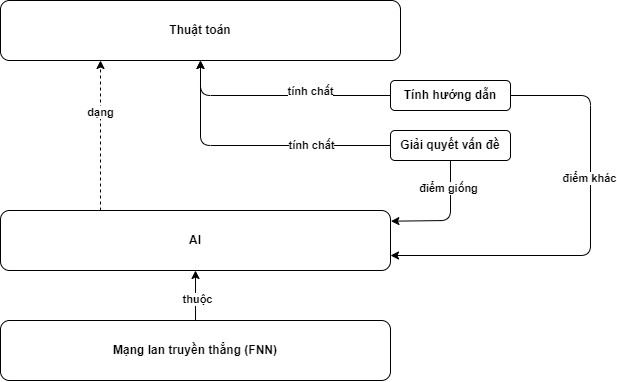
\includegraphics[scale=0.6]{figures/ai_fnn_algorithm.png}
		\caption{Mối quan hệ giữa AI, thuật toán và mạng lan truyền thẳng (FNN). AI giống thuật toán là đều dùng để giải quyết vấn đề nhưng khác nhau ở bước hướng dẫn. Mặt khác FNN là một con của AI, AI có những thuộc tính trên thì mạng FNN cũng sẽ có.}
		\label{fig:ai_fnn_algo_relationship}
	\end{figure}  
	
	Như vậy thông qua sơ đồ trên, ta biết được FNN sẽ có những tính chất mà AI có. Nhờ vậy, tìm hiểu thêm về mạng này cũng sẽ góp phần hiểu thêm về thuật toán.
	
\subsection{FNN}
	Để cho câu trả lời cho câu hỏi chủ đề được trọn vẹn. Hãy tìm hiểu sơ qua về mạng FNN.
	
	FNN là một cấu trúc cơ bản và quan trọng trong học sâu (Deep Learning). Dựa trên tiền đề này mà nhiều mạng với kiến trúc tiên tiến hơn được ra đời. Ngoài ra tính chất của FNN là thông tin chỉ lan truyền theo một chiều duy nhất xuyên suốt và không có vòng lặp.
	
	FNN là một dạng của mạng thần kinh nhân tạo (Artificial Neural Network). Tất có nghĩa, FNN là một tập hợp các neuron và sự kết nối giữa chúng.
	
	Mặt khác, do mang trong mình tính chất của một thuật toán nên để có thể diễn giải sang mã lập trình được thì cần thông qua một cây cầu mang tên \textbf{toán học}. Trong bối cảnh này, toán học dùng để mô phỏng hành vi của một đơn vị neuron và hành vi của một tập các neuron được kết nối với nhau. Về cụ thể:
	\begin{itemize}
		\item một đơn vị neuron có hành vi: nhận tín hiệu từ nhiều nguồn, tiến hành tổng hợp và đưa ra kết quả. Ở mặt này có thể dùng hàm số để mô phỏng hành vi. Cụ thể hơn, trong trường hợp này là hàm phi tuyến với công thức:
		
		\begin{equation}
			 f(x) = \sigma(w_0 + \sum_{i=1}^{n} w_{i} * x_{i})
		\end{equation}
		
		Hệ số $w_0$ là hệ số đền bù (bias) và $w_i$ là các trọng số kích hoạt ứng với đầu vào $x_i$, và $n$ là số lượng đầu vào.
		
		\item một tập hợp neuron. Mang hành vi kế thừa của các neuron nhưng sẽ nhận nhiều đầu vào và cho ra nhiều kết quả. Để làm được điều này, ma trận được dùng để mô phỏng hành vi. Ngoài ra việc dùng ma trận thay vì tập trung vào mô phỏng từng đơn vị sẽ đem đến hiệu quả tính toán tốt hơn.
		
		\begin{equation}
			f(X) = \sigma(W^TX + B)
		\end{equation}
		
		Với $X$ là một tập đầu vào với kích thước $ \text{data\_points} \times \text{input\_dim} $, $X$ là một ma trận. $W$ là tập trọng số với kích thước $ \text{output\_dim} \times \text{input\_dim} $. $W$ cũng là một ma trận và $W^T$ là ma trận chuyển vị. $B$ đóng vai trò như hệ số bù với kích thước $1 \times \text{output\_dim} $.
	\end{itemize}

	Ở mặt hình tượng, đây là sơ đồ của mạng FNN.
	
	\begin{figure}[h]
		\centering
		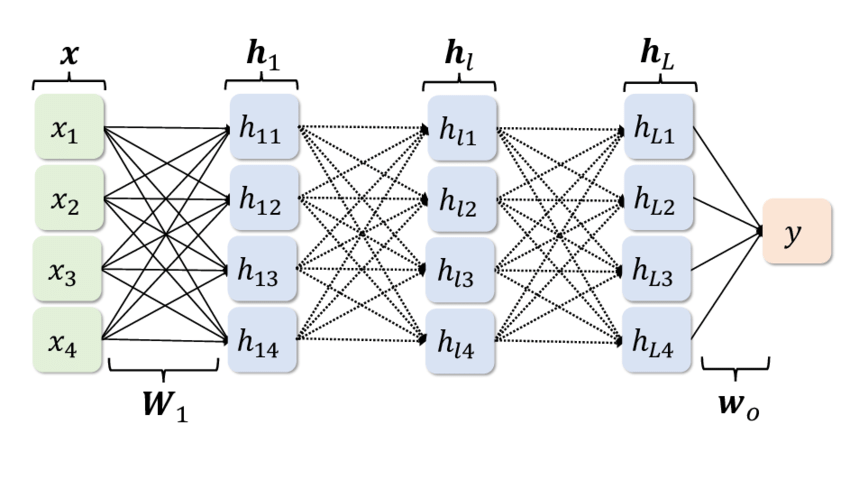
\includegraphics[scale=0.3]{figures/fnn.illustration.png}
		\caption{Ảnh minh hoạ cho mạng FNN \cite{fnn_figure}. Gồm các trọng số và các đơn vị. Mạng này có 5 tầng gồm 1 tầng đầu vào, 1 tầng đầu ra và 3 tầng ẩn.}
		\label{fig:fnn_illustration}
	\end{figure}
	
\noindent
Qua quá trình phân tích và tìm hiểu về mạng FNN, bài viết làm rõ thêm về mối quan hệ của các đối tượng. Qua đó khẳng định thêm về vị trí đứng của \textbf{toán học} trong câu hỏi \hyperlink{main_question}{"Người lập trình lấy ý tưởng từ đâu?"}